% Created by tikzDevice version 0.6.1 on 2016-04-19 18:32:53
% !TEX encoding = UTF-8 Unicode
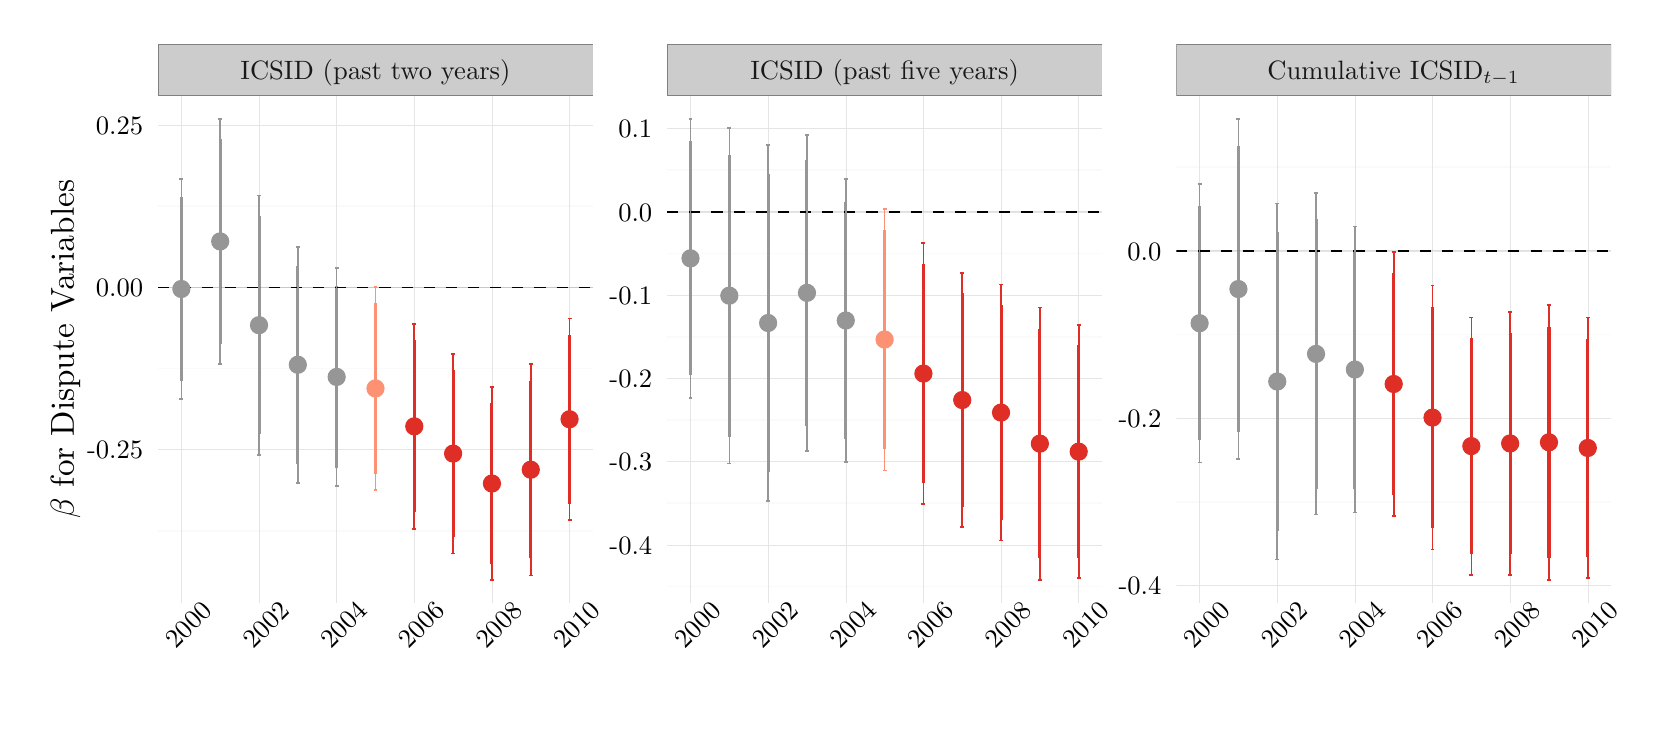
\begin{tikzpicture}[x=1pt,y=1pt]
\definecolor[named]{drawColor}{rgb}{0.00,0.00,0.00}
\definecolor[named]{fillColor}{rgb}{1.00,1.00,1.00}
\fill[color=fillColor,] (0,0) rectangle (578.16,252.94);
\begin{scope}
\path[clip] (  0.00,  0.00) rectangle (578.16,252.94);
\end{scope}
\begin{scope}
\path[clip] (  0.00,  0.00) rectangle (578.16,252.94);
\end{scope}
\begin{scope}
\path[clip] (  0.00,  0.00) rectangle (578.16,252.94);
\end{scope}
\begin{scope}
\path[clip] (  0.00,  0.00) rectangle (578.16,252.94);
\end{scope}
\begin{scope}
\path[clip] (  0.00,  0.00) rectangle (578.16,252.94);
\end{scope}
\begin{scope}
\path[clip] (  0.00,  0.00) rectangle (578.16,252.94);
\end{scope}
\begin{scope}
\path[clip] (  0.00,  0.00) rectangle (578.16,252.94);
\end{scope}
\begin{scope}
\path[clip] (  0.00,  0.00) rectangle (578.16,252.94);
\end{scope}
\begin{scope}
\path[clip] (  0.00,  0.00) rectangle (578.16,252.94);
\end{scope}
\begin{scope}
\path[clip] (  0.00,  0.00) rectangle (578.16,252.94);
\end{scope}
\begin{scope}
\path[clip] (  0.00,  0.00) rectangle (578.16,252.94);
\end{scope}
\begin{scope}
\path[clip] (  0.00,  0.00) rectangle (578.16,252.94);
\end{scope}
\begin{scope}
\path[clip] (  0.00,  0.00) rectangle (578.16,252.94);
\end{scope}
\begin{scope}
\path[clip] (  0.00,  0.00) rectangle (578.16,252.94);
\end{scope}
\begin{scope}
\path[clip] (  0.00,  0.00) rectangle (578.16,252.94);
\end{scope}
\begin{scope}
\path[clip] (  0.00,  0.00) rectangle (578.16,252.94);
\end{scope}
\begin{scope}
\path[clip] (  0.00,  0.00) rectangle (578.16,252.94);
\end{scope}
\begin{scope}
\path[clip] (  0.00,  0.00) rectangle (578.16,252.94);
\end{scope}
\begin{scope}
\path[clip] (  0.00,  0.00) rectangle (578.16,252.94);
\definecolor[named]{drawColor}{rgb}{1.00,1.00,1.00}
\definecolor[named]{fillColor}{rgb}{1.00,1.00,1.00}

\draw[color=drawColor,line width= 0.6pt,line cap=round,line join=round,fill=fillColor,] ( -0.00,  0.00) rectangle (578.16,252.94);
\end{scope}
\begin{scope}
\path[clip] (  0.00,  0.00) rectangle (578.16,252.94);
\end{scope}
\begin{scope}
\path[clip] ( 47.13, 45.11) rectangle (204.23,228.33);
\definecolor[named]{fillColor}{rgb}{1.00,1.00,1.00}

\draw[fill=fillColor,draw opacity=0.00,] ( 47.13, 45.11) rectangle (204.23,228.33);
\definecolor[named]{drawColor}{rgb}{0.98,0.98,0.98}

\draw[color=drawColor,line width= 0.6pt,line join=round,fill opacity=0.00,] ( 47.13, 71.11) --
	(204.23, 71.11);

\draw[color=drawColor,line width= 0.6pt,line join=round,fill opacity=0.00,] ( 47.13,129.76) --
	(204.23,129.76);

\draw[color=drawColor,line width= 0.6pt,line join=round,fill opacity=0.00,] ( 47.13,188.41) --
	(204.23,188.41);
\definecolor[named]{drawColor}{rgb}{0.90,0.90,0.90}

\draw[color=drawColor,line width= 0.2pt,line join=round,fill opacity=0.00,] ( 47.13,100.44) --
	(204.23,100.44);

\draw[color=drawColor,line width= 0.2pt,line join=round,fill opacity=0.00,] ( 47.13,159.09) --
	(204.23,159.09);

\draw[color=drawColor,line width= 0.2pt,line join=round,fill opacity=0.00,] ( 47.13,217.74) --
	(204.23,217.74);

\draw[color=drawColor,line width= 0.2pt,line join=round,fill opacity=0.00,] ( 55.54, 45.11) --
	( 55.54,228.33);

\draw[color=drawColor,line width= 0.2pt,line join=round,fill opacity=0.00,] ( 83.60, 45.11) --
	( 83.60,228.33);

\draw[color=drawColor,line width= 0.2pt,line join=round,fill opacity=0.00,] (111.65, 45.11) --
	(111.65,228.33);

\draw[color=drawColor,line width= 0.2pt,line join=round,fill opacity=0.00,] (139.70, 45.11) --
	(139.70,228.33);

\draw[color=drawColor,line width= 0.2pt,line join=round,fill opacity=0.00,] (167.76, 45.11) --
	(167.76,228.33);

\draw[color=drawColor,line width= 0.2pt,line join=round,fill opacity=0.00,] (195.81, 45.11) --
	(195.81,228.33);
\definecolor[named]{drawColor}{rgb}{0.59,0.59,0.59}
\definecolor[named]{fillColor}{rgb}{0.59,0.59,0.59}

\draw[color=drawColor,line width= 0.3pt,line join=round,fill=fillColor,fill opacity=0.30,draw opacity=0.30,] ( 55.54,118.77) -- ( 55.54,198.25);

\draw[color=drawColor,line width= 0.3pt,line join=round,fill=fillColor,fill opacity=0.30,draw opacity=0.30,] ( 69.57,131.39) -- ( 69.57,220.01);

\draw[color=drawColor,line width= 0.3pt,line join=round,fill=fillColor,fill opacity=0.30,draw opacity=0.30,] ( 83.60, 98.54) -- ( 83.60,192.32);

\draw[color=drawColor,line width= 0.3pt,line join=round,fill=fillColor,fill opacity=0.30,draw opacity=0.30,] ( 97.62, 88.47) -- ( 97.62,173.80);

\draw[color=drawColor,line width= 0.3pt,line join=round,fill=fillColor,fill opacity=0.30,draw opacity=0.30,] (111.65, 87.39) -- (111.65,166.06);
\definecolor[named]{drawColor}{rgb}{0.99,0.57,0.45}
\definecolor[named]{fillColor}{rgb}{0.99,0.57,0.45}

\draw[color=drawColor,line width= 0.3pt,line join=round,fill=fillColor,fill opacity=0.30,draw opacity=0.30,] (125.68, 85.90) -- (125.68,159.23);
\definecolor[named]{drawColor}{rgb}{0.87,0.18,0.15}
\definecolor[named]{fillColor}{rgb}{0.87,0.18,0.15}

\draw[color=drawColor,line width= 0.3pt,line join=round,fill=fillColor,fill opacity=0.30,draw opacity=0.30,] (139.70, 71.80) -- (139.70,145.96);

\draw[color=drawColor,line width= 0.3pt,line join=round,fill=fillColor,fill opacity=0.30,draw opacity=0.30,] (153.73, 62.95) -- (153.73,135.10);

\draw[color=drawColor,line width= 0.3pt,line join=round,fill=fillColor,fill opacity=0.30,draw opacity=0.30,] (167.76, 53.44) -- (167.76,123.00);

\draw[color=drawColor,line width= 0.3pt,line join=round,fill=fillColor,fill opacity=0.30,draw opacity=0.30,] (181.79, 55.04) -- (181.79,131.37);

\draw[color=drawColor,line width= 0.3pt,line join=round,fill=fillColor,fill opacity=0.30,draw opacity=0.30,] (195.81, 75.10) -- (195.81,147.80);
\definecolor[named]{drawColor}{rgb}{0.59,0.59,0.59}
\definecolor[named]{fillColor}{rgb}{0.59,0.59,0.59}

\draw[color=drawColor,line width= 1.1pt,line join=round,fill=fillColor,] ( 55.54,125.15) -- ( 55.54,191.86);

\draw[color=drawColor,line width= 1.1pt,line join=round,fill=fillColor,] ( 69.57,138.51) -- ( 69.57,212.88);

\draw[color=drawColor,line width= 1.1pt,line join=round,fill=fillColor,] ( 83.60,106.07) -- ( 83.60,184.78);

\draw[color=drawColor,line width= 1.1pt,line join=round,fill=fillColor,] ( 97.62, 95.33) -- ( 97.62,166.94);

\draw[color=drawColor,line width= 1.1pt,line join=round,fill=fillColor,] (111.65, 93.72) -- (111.65,159.73);
\definecolor[named]{drawColor}{rgb}{0.99,0.57,0.45}
\definecolor[named]{fillColor}{rgb}{0.99,0.57,0.45}

\draw[color=drawColor,line width= 1.1pt,line join=round,fill=fillColor,] (125.68, 91.80) -- (125.68,153.34);
\definecolor[named]{drawColor}{rgb}{0.87,0.18,0.15}
\definecolor[named]{fillColor}{rgb}{0.87,0.18,0.15}

\draw[color=drawColor,line width= 1.1pt,line join=round,fill=fillColor,] (139.70, 77.76) -- (139.70,140.00);

\draw[color=drawColor,line width= 1.1pt,line join=round,fill=fillColor,] (153.73, 68.75) -- (153.73,129.30);

\draw[color=drawColor,line width= 1.1pt,line join=round,fill=fillColor,] (167.76, 59.03) -- (167.76,117.40);

\draw[color=drawColor,line width= 1.1pt,line join=round,fill=fillColor,] (181.79, 61.18) -- (181.79,125.23);

\draw[color=drawColor,line width= 1.1pt,line join=round,fill=fillColor,] (195.81, 80.95) -- (195.81,141.95);
\definecolor[named]{drawColor}{rgb}{0.00,0.00,0.00}
\definecolor[named]{fillColor}{rgb}{0.00,0.00,0.00}

\draw[color=drawColor,line width= 0.6pt,dash pattern=on 4pt off 4pt ,line join=round,fill=fillColor,] ( 47.13,159.09) -- (204.23,159.09);
\definecolor[named]{drawColor}{rgb}{0.59,0.59,0.59}
\definecolor[named]{fillColor}{rgb}{0.59,0.59,0.59}

\draw[color=drawColor,line width= 0.4pt,line cap=round,line join=round,fill=fillColor,] ( 55.54,158.51) circle (  3.09);

\draw[color=drawColor,line width= 0.4pt,line cap=round,line join=round,fill=fillColor,] ( 69.57,175.70) circle (  3.09);

\draw[color=drawColor,line width= 0.4pt,line cap=round,line join=round,fill=fillColor,] ( 83.60,145.43) circle (  3.09);

\draw[color=drawColor,line width= 0.4pt,line cap=round,line join=round,fill=fillColor,] ( 97.62,131.13) circle (  3.09);

\draw[color=drawColor,line width= 0.4pt,line cap=round,line join=round,fill=fillColor,] (111.65,126.73) circle (  3.09);
\definecolor[named]{drawColor}{rgb}{0.99,0.57,0.45}
\definecolor[named]{fillColor}{rgb}{0.99,0.57,0.45}

\draw[color=drawColor,line width= 0.4pt,line cap=round,line join=round,fill=fillColor,] (125.68,122.57) circle (  3.09);
\definecolor[named]{drawColor}{rgb}{0.87,0.18,0.15}
\definecolor[named]{fillColor}{rgb}{0.87,0.18,0.15}

\draw[color=drawColor,line width= 0.4pt,line cap=round,line join=round,fill=fillColor,] (139.70,108.88) circle (  3.09);

\draw[color=drawColor,line width= 0.4pt,line cap=round,line join=round,fill=fillColor,] (153.73, 99.03) circle (  3.09);

\draw[color=drawColor,line width= 0.4pt,line cap=round,line join=round,fill=fillColor,] (167.76, 88.22) circle (  3.09);

\draw[color=drawColor,line width= 0.4pt,line cap=round,line join=round,fill=fillColor,] (181.79, 93.20) circle (  3.09);

\draw[color=drawColor,line width= 0.4pt,line cap=round,line join=round,fill=fillColor,] (195.81,111.45) circle (  3.09);
\definecolor[named]{drawColor}{rgb}{0.59,0.59,0.59}
\definecolor[named]{fillColor}{rgb}{0.59,0.59,0.59}

\draw[color=drawColor,line width= 0.6pt,line join=round,] ( 54.84,198.25) --
	( 56.24,198.25);

\draw[color=drawColor,line width= 0.6pt,line join=round,] ( 55.54,198.25) --
	( 55.54,118.77);

\draw[color=drawColor,line width= 0.6pt,line join=round,] ( 54.84,118.77) --
	( 56.24,118.77);

\draw[color=drawColor,line width= 0.6pt,line join=round,] ( 68.87,220.01) --
	( 70.27,220.01);

\draw[color=drawColor,line width= 0.6pt,line join=round,] ( 69.57,220.01) --
	( 69.57,131.39);

\draw[color=drawColor,line width= 0.6pt,line join=round,] ( 68.87,131.39) --
	( 70.27,131.39);

\draw[color=drawColor,line width= 0.6pt,line join=round,] ( 82.90,192.32) --
	( 84.30,192.32);

\draw[color=drawColor,line width= 0.6pt,line join=round,] ( 83.60,192.32) --
	( 83.60, 98.54);

\draw[color=drawColor,line width= 0.6pt,line join=round,] ( 82.90, 98.54) --
	( 84.30, 98.54);

\draw[color=drawColor,line width= 0.6pt,line join=round,] ( 96.92,173.80) --
	( 98.33,173.80);

\draw[color=drawColor,line width= 0.6pt,line join=round,] ( 97.62,173.80) --
	( 97.62, 88.47);

\draw[color=drawColor,line width= 0.6pt,line join=round,] ( 96.92, 88.47) --
	( 98.33, 88.47);

\draw[color=drawColor,line width= 0.6pt,line join=round,] (110.95,166.06) --
	(112.35,166.06);

\draw[color=drawColor,line width= 0.6pt,line join=round,] (111.65,166.06) --
	(111.65, 87.39);

\draw[color=drawColor,line width= 0.6pt,line join=round,] (110.95, 87.39) --
	(112.35, 87.39);
\definecolor[named]{drawColor}{rgb}{0.99,0.57,0.45}
\definecolor[named]{fillColor}{rgb}{0.99,0.57,0.45}

\draw[color=drawColor,line width= 0.6pt,line join=round,] (124.98,159.23) --
	(126.38,159.23);

\draw[color=drawColor,line width= 0.6pt,line join=round,] (125.68,159.23) --
	(125.68, 85.90);

\draw[color=drawColor,line width= 0.6pt,line join=round,] (124.98, 85.90) --
	(126.38, 85.90);
\definecolor[named]{drawColor}{rgb}{0.87,0.18,0.15}
\definecolor[named]{fillColor}{rgb}{0.87,0.18,0.15}

\draw[color=drawColor,line width= 0.6pt,line join=round,] (139.00,145.96) --
	(140.41,145.96);

\draw[color=drawColor,line width= 0.6pt,line join=round,] (139.70,145.96) --
	(139.70, 71.80);

\draw[color=drawColor,line width= 0.6pt,line join=round,] (139.00, 71.80) --
	(140.41, 71.80);

\draw[color=drawColor,line width= 0.6pt,line join=round,] (153.03,135.10) --
	(154.43,135.10);

\draw[color=drawColor,line width= 0.6pt,line join=round,] (153.73,135.10) --
	(153.73, 62.95);

\draw[color=drawColor,line width= 0.6pt,line join=round,] (153.03, 62.95) --
	(154.43, 62.95);

\draw[color=drawColor,line width= 0.6pt,line join=round,] (167.06,123.00) --
	(168.46,123.00);

\draw[color=drawColor,line width= 0.6pt,line join=round,] (167.76,123.00) --
	(167.76, 53.44);

\draw[color=drawColor,line width= 0.6pt,line join=round,] (167.06, 53.44) --
	(168.46, 53.44);

\draw[color=drawColor,line width= 0.6pt,line join=round,] (181.08,131.37) --
	(182.49,131.37);

\draw[color=drawColor,line width= 0.6pt,line join=round,] (181.79,131.37) --
	(181.79, 55.04);

\draw[color=drawColor,line width= 0.6pt,line join=round,] (181.08, 55.04) --
	(182.49, 55.04);

\draw[color=drawColor,line width= 0.6pt,line join=round,] (195.11,147.80) --
	(196.51,147.80);

\draw[color=drawColor,line width= 0.6pt,line join=round,] (195.81,147.80) --
	(195.81, 75.10);

\draw[color=drawColor,line width= 0.6pt,line join=round,] (195.11, 75.10) --
	(196.51, 75.10);
\end{scope}
\begin{scope}
\path[clip] (  0.00,  0.00) rectangle (578.16,252.94);
\end{scope}
\begin{scope}
\path[clip] (231.09, 45.11) rectangle (388.19,228.33);
\definecolor[named]{fillColor}{rgb}{1.00,1.00,1.00}

\draw[fill=fillColor,draw opacity=0.00,] (231.09, 45.11) rectangle (388.19,228.33);
\definecolor[named]{drawColor}{rgb}{0.98,0.98,0.98}

\draw[color=drawColor,line width= 0.6pt,line join=round,fill opacity=0.00,] (231.09, 50.98) --
	(388.19, 50.98);

\draw[color=drawColor,line width= 0.6pt,line join=round,fill opacity=0.00,] (231.09, 81.06) --
	(388.19, 81.06);

\draw[color=drawColor,line width= 0.6pt,line join=round,fill opacity=0.00,] (231.09,111.14) --
	(388.19,111.14);

\draw[color=drawColor,line width= 0.6pt,line join=round,fill opacity=0.00,] (231.09,141.23) --
	(388.19,141.23);

\draw[color=drawColor,line width= 0.6pt,line join=round,fill opacity=0.00,] (231.09,171.31) --
	(388.19,171.31);

\draw[color=drawColor,line width= 0.6pt,line join=round,fill opacity=0.00,] (231.09,201.39) --
	(388.19,201.39);
\definecolor[named]{drawColor}{rgb}{0.90,0.90,0.90}

\draw[color=drawColor,line width= 0.2pt,line join=round,fill opacity=0.00,] (231.09, 66.02) --
	(388.19, 66.02);

\draw[color=drawColor,line width= 0.2pt,line join=round,fill opacity=0.00,] (231.09, 96.10) --
	(388.19, 96.10);

\draw[color=drawColor,line width= 0.2pt,line join=round,fill opacity=0.00,] (231.09,126.18) --
	(388.19,126.18);

\draw[color=drawColor,line width= 0.2pt,line join=round,fill opacity=0.00,] (231.09,156.27) --
	(388.19,156.27);

\draw[color=drawColor,line width= 0.2pt,line join=round,fill opacity=0.00,] (231.09,186.35) --
	(388.19,186.35);

\draw[color=drawColor,line width= 0.2pt,line join=round,fill opacity=0.00,] (231.09,216.43) --
	(388.19,216.43);

\draw[color=drawColor,line width= 0.2pt,line join=round,fill opacity=0.00,] (239.51, 45.11) --
	(239.51,228.33);

\draw[color=drawColor,line width= 0.2pt,line join=round,fill opacity=0.00,] (267.56, 45.11) --
	(267.56,228.33);

\draw[color=drawColor,line width= 0.2pt,line join=round,fill opacity=0.00,] (295.62, 45.11) --
	(295.62,228.33);

\draw[color=drawColor,line width= 0.2pt,line join=round,fill opacity=0.00,] (323.67, 45.11) --
	(323.67,228.33);

\draw[color=drawColor,line width= 0.2pt,line join=round,fill opacity=0.00,] (351.72, 45.11) --
	(351.72,228.33);

\draw[color=drawColor,line width= 0.2pt,line join=round,fill opacity=0.00,] (379.78, 45.11) --
	(379.78,228.33);
\definecolor[named]{drawColor}{rgb}{0.59,0.59,0.59}
\definecolor[named]{fillColor}{rgb}{0.59,0.59,0.59}

\draw[color=drawColor,line width= 0.3pt,line join=round,fill=fillColor,fill opacity=0.30,draw opacity=0.30,] (239.51,119.16) -- (239.51,220.01);

\draw[color=drawColor,line width= 0.3pt,line join=round,fill=fillColor,fill opacity=0.30,draw opacity=0.30,] (253.54, 95.44) -- (253.54,216.76);

\draw[color=drawColor,line width= 0.3pt,line join=round,fill=fillColor,fill opacity=0.30,draw opacity=0.30,] (267.56, 81.90) -- (267.56,210.54);

\draw[color=drawColor,line width= 0.3pt,line join=round,fill=fillColor,fill opacity=0.30,draw opacity=0.30,] (281.59, 99.99) -- (281.59,214.25);

\draw[color=drawColor,line width= 0.3pt,line join=round,fill=fillColor,fill opacity=0.30,draw opacity=0.30,] (295.62, 96.02) -- (295.62,198.24);
\definecolor[named]{drawColor}{rgb}{0.99,0.57,0.45}
\definecolor[named]{fillColor}{rgb}{0.99,0.57,0.45}

\draw[color=drawColor,line width= 0.3pt,line join=round,fill=fillColor,fill opacity=0.30,draw opacity=0.30,] (309.64, 92.97) -- (309.64,187.53);
\definecolor[named]{drawColor}{rgb}{0.87,0.18,0.15}
\definecolor[named]{fillColor}{rgb}{0.87,0.18,0.15}

\draw[color=drawColor,line width= 0.3pt,line join=round,fill=fillColor,fill opacity=0.30,draw opacity=0.30,] (323.67, 80.85) -- (323.67,175.06);

\draw[color=drawColor,line width= 0.3pt,line join=round,fill=fillColor,fill opacity=0.30,draw opacity=0.30,] (337.70, 72.47) -- (337.70,164.31);

\draw[color=drawColor,line width= 0.3pt,line join=round,fill=fillColor,fill opacity=0.30,draw opacity=0.30,] (351.72, 67.57) -- (351.72,160.14);

\draw[color=drawColor,line width= 0.3pt,line join=round,fill=fillColor,fill opacity=0.30,draw opacity=0.30,] (365.75, 53.44) -- (365.75,151.82);

\draw[color=drawColor,line width= 0.3pt,line join=round,fill=fillColor,fill opacity=0.30,draw opacity=0.30,] (379.78, 54.03) -- (379.78,145.45);
\definecolor[named]{drawColor}{rgb}{0.59,0.59,0.59}
\definecolor[named]{fillColor}{rgb}{0.59,0.59,0.59}

\draw[color=drawColor,line width= 1.1pt,line join=round,fill=fillColor,] (239.51,127.27) -- (239.51,211.90);

\draw[color=drawColor,line width= 1.1pt,line join=round,fill=fillColor,] (253.54,105.19) -- (253.54,207.01);

\draw[color=drawColor,line width= 1.1pt,line join=round,fill=fillColor,] (267.56, 92.24) -- (267.56,200.20);

\draw[color=drawColor,line width= 1.1pt,line join=round,fill=fillColor,] (281.59,109.18) -- (281.59,205.06);

\draw[color=drawColor,line width= 1.1pt,line join=round,fill=fillColor,] (295.62,104.23) -- (295.62,190.02);
\definecolor[named]{drawColor}{rgb}{0.99,0.57,0.45}
\definecolor[named]{fillColor}{rgb}{0.99,0.57,0.45}

\draw[color=drawColor,line width= 1.1pt,line join=round,fill=fillColor,] (309.64,100.57) -- (309.64,179.93);
\definecolor[named]{drawColor}{rgb}{0.87,0.18,0.15}
\definecolor[named]{fillColor}{rgb}{0.87,0.18,0.15}

\draw[color=drawColor,line width= 1.1pt,line join=round,fill=fillColor,] (323.67, 88.42) -- (323.67,167.49);

\draw[color=drawColor,line width= 1.1pt,line join=round,fill=fillColor,] (337.70, 79.85) -- (337.70,156.92);

\draw[color=drawColor,line width= 1.1pt,line join=round,fill=fillColor,] (351.72, 75.01) -- (351.72,152.70);

\draw[color=drawColor,line width= 1.1pt,line join=round,fill=fillColor,] (365.75, 61.35) -- (365.75,143.91);

\draw[color=drawColor,line width= 1.1pt,line join=round,fill=fillColor,] (379.78, 61.38) -- (379.78,138.10);
\definecolor[named]{drawColor}{rgb}{0.00,0.00,0.00}
\definecolor[named]{fillColor}{rgb}{0.00,0.00,0.00}

\draw[color=drawColor,line width= 0.6pt,dash pattern=on 4pt off 4pt ,line join=round,fill=fillColor,] (231.09,186.35) -- (388.19,186.35);
\definecolor[named]{drawColor}{rgb}{0.59,0.59,0.59}
\definecolor[named]{fillColor}{rgb}{0.59,0.59,0.59}

\draw[color=drawColor,line width= 0.4pt,line cap=round,line join=round,fill=fillColor,] (239.51,169.58) circle (  3.09);

\draw[color=drawColor,line width= 0.4pt,line cap=round,line join=round,fill=fillColor,] (253.54,156.10) circle (  3.09);

\draw[color=drawColor,line width= 0.4pt,line cap=round,line join=round,fill=fillColor,] (267.56,146.22) circle (  3.09);

\draw[color=drawColor,line width= 0.4pt,line cap=round,line join=round,fill=fillColor,] (281.59,157.12) circle (  3.09);

\draw[color=drawColor,line width= 0.4pt,line cap=round,line join=round,fill=fillColor,] (295.62,147.13) circle (  3.09);
\definecolor[named]{drawColor}{rgb}{0.99,0.57,0.45}
\definecolor[named]{fillColor}{rgb}{0.99,0.57,0.45}

\draw[color=drawColor,line width= 0.4pt,line cap=round,line join=round,fill=fillColor,] (309.64,140.25) circle (  3.09);
\definecolor[named]{drawColor}{rgb}{0.87,0.18,0.15}
\definecolor[named]{fillColor}{rgb}{0.87,0.18,0.15}

\draw[color=drawColor,line width= 0.4pt,line cap=round,line join=round,fill=fillColor,] (323.67,127.95) circle (  3.09);

\draw[color=drawColor,line width= 0.4pt,line cap=round,line join=round,fill=fillColor,] (337.70,118.39) circle (  3.09);

\draw[color=drawColor,line width= 0.4pt,line cap=round,line join=round,fill=fillColor,] (351.72,113.85) circle (  3.09);

\draw[color=drawColor,line width= 0.4pt,line cap=round,line join=round,fill=fillColor,] (365.75,102.63) circle (  3.09);

\draw[color=drawColor,line width= 0.4pt,line cap=round,line join=round,fill=fillColor,] (379.78, 99.74) circle (  3.09);
\definecolor[named]{drawColor}{rgb}{0.59,0.59,0.59}
\definecolor[named]{fillColor}{rgb}{0.59,0.59,0.59}

\draw[color=drawColor,line width= 0.6pt,line join=round,] (238.81,220.01) --
	(240.21,220.01);

\draw[color=drawColor,line width= 0.6pt,line join=round,] (239.51,220.01) --
	(239.51,119.16);

\draw[color=drawColor,line width= 0.6pt,line join=round,] (238.81,119.16) --
	(240.21,119.16);

\draw[color=drawColor,line width= 0.6pt,line join=round,] (252.83,216.76) --
	(254.24,216.76);

\draw[color=drawColor,line width= 0.6pt,line join=round,] (253.54,216.76) --
	(253.54, 95.44);

\draw[color=drawColor,line width= 0.6pt,line join=round,] (252.83, 95.44) --
	(254.24, 95.44);

\draw[color=drawColor,line width= 0.6pt,line join=round,] (266.86,210.54) --
	(268.26,210.54);

\draw[color=drawColor,line width= 0.6pt,line join=round,] (267.56,210.54) --
	(267.56, 81.90);

\draw[color=drawColor,line width= 0.6pt,line join=round,] (266.86, 81.90) --
	(268.26, 81.90);

\draw[color=drawColor,line width= 0.6pt,line join=round,] (280.89,214.25) --
	(282.29,214.25);

\draw[color=drawColor,line width= 0.6pt,line join=round,] (281.59,214.25) --
	(281.59, 99.99);

\draw[color=drawColor,line width= 0.6pt,line join=round,] (280.89, 99.99) --
	(282.29, 99.99);

\draw[color=drawColor,line width= 0.6pt,line join=round,] (294.91,198.24) --
	(296.32,198.24);

\draw[color=drawColor,line width= 0.6pt,line join=round,] (295.62,198.24) --
	(295.62, 96.02);

\draw[color=drawColor,line width= 0.6pt,line join=round,] (294.91, 96.02) --
	(296.32, 96.02);
\definecolor[named]{drawColor}{rgb}{0.99,0.57,0.45}
\definecolor[named]{fillColor}{rgb}{0.99,0.57,0.45}

\draw[color=drawColor,line width= 0.6pt,line join=round,] (308.94,187.53) --
	(310.34,187.53);

\draw[color=drawColor,line width= 0.6pt,line join=round,] (309.64,187.53) --
	(309.64, 92.97);

\draw[color=drawColor,line width= 0.6pt,line join=round,] (308.94, 92.97) --
	(310.34, 92.97);
\definecolor[named]{drawColor}{rgb}{0.87,0.18,0.15}
\definecolor[named]{fillColor}{rgb}{0.87,0.18,0.15}

\draw[color=drawColor,line width= 0.6pt,line join=round,] (322.97,175.06) --
	(324.37,175.06);

\draw[color=drawColor,line width= 0.6pt,line join=round,] (323.67,175.06) --
	(323.67, 80.85);

\draw[color=drawColor,line width= 0.6pt,line join=round,] (322.97, 80.85) --
	(324.37, 80.85);

\draw[color=drawColor,line width= 0.6pt,line join=round,] (337.00,164.31) --
	(338.40,164.31);

\draw[color=drawColor,line width= 0.6pt,line join=round,] (337.70,164.31) --
	(337.70, 72.47);

\draw[color=drawColor,line width= 0.6pt,line join=round,] (337.00, 72.47) --
	(338.40, 72.47);

\draw[color=drawColor,line width= 0.6pt,line join=round,] (351.02,160.14) --
	(352.43,160.14);

\draw[color=drawColor,line width= 0.6pt,line join=round,] (351.72,160.14) --
	(351.72, 67.57);

\draw[color=drawColor,line width= 0.6pt,line join=round,] (351.02, 67.57) --
	(352.43, 67.57);

\draw[color=drawColor,line width= 0.6pt,line join=round,] (365.05,151.82) --
	(366.45,151.82);

\draw[color=drawColor,line width= 0.6pt,line join=round,] (365.75,151.82) --
	(365.75, 53.44);

\draw[color=drawColor,line width= 0.6pt,line join=round,] (365.05, 53.44) --
	(366.45, 53.44);

\draw[color=drawColor,line width= 0.6pt,line join=round,] (379.08,145.45) --
	(380.48,145.45);

\draw[color=drawColor,line width= 0.6pt,line join=round,] (379.78,145.45) --
	(379.78, 54.03);

\draw[color=drawColor,line width= 0.6pt,line join=round,] (379.08, 54.03) --
	(380.48, 54.03);
\end{scope}
\begin{scope}
\path[clip] (  0.00,  0.00) rectangle (578.16,252.94);
\end{scope}
\begin{scope}
\path[clip] (415.06, 45.11) rectangle (572.16,228.33);
\definecolor[named]{fillColor}{rgb}{1.00,1.00,1.00}

\draw[fill=fillColor,draw opacity=0.00,] (415.06, 45.11) rectangle (572.16,228.33);
\definecolor[named]{drawColor}{rgb}{0.98,0.98,0.98}

\draw[color=drawColor,line width= 0.6pt,line join=round,fill opacity=0.00,] (415.06, 81.53) --
	(572.16, 81.53);

\draw[color=drawColor,line width= 0.6pt,line join=round,fill opacity=0.00,] (415.06,142.02) --
	(572.16,142.02);

\draw[color=drawColor,line width= 0.6pt,line join=round,fill opacity=0.00,] (415.06,202.52) --
	(572.16,202.52);
\definecolor[named]{drawColor}{rgb}{0.90,0.90,0.90}

\draw[color=drawColor,line width= 0.2pt,line join=round,fill opacity=0.00,] (415.06, 51.28) --
	(572.16, 51.28);

\draw[color=drawColor,line width= 0.2pt,line join=round,fill opacity=0.00,] (415.06,111.78) --
	(572.16,111.78);

\draw[color=drawColor,line width= 0.2pt,line join=round,fill opacity=0.00,] (415.06,172.27) --
	(572.16,172.27);

\draw[color=drawColor,line width= 0.2pt,line join=round,fill opacity=0.00,] (423.47, 45.11) --
	(423.47,228.33);

\draw[color=drawColor,line width= 0.2pt,line join=round,fill opacity=0.00,] (451.53, 45.11) --
	(451.53,228.33);

\draw[color=drawColor,line width= 0.2pt,line join=round,fill opacity=0.00,] (479.58, 45.11) --
	(479.58,228.33);

\draw[color=drawColor,line width= 0.2pt,line join=round,fill opacity=0.00,] (507.64, 45.11) --
	(507.64,228.33);

\draw[color=drawColor,line width= 0.2pt,line join=round,fill opacity=0.00,] (535.69, 45.11) --
	(535.69,228.33);

\draw[color=drawColor,line width= 0.2pt,line join=round,fill opacity=0.00,] (563.74, 45.11) --
	(563.74,228.33);
\definecolor[named]{drawColor}{rgb}{0.59,0.59,0.59}
\definecolor[named]{fillColor}{rgb}{0.59,0.59,0.59}

\draw[color=drawColor,line width= 0.3pt,line join=round,fill=fillColor,fill opacity=0.30,draw opacity=0.30,] (423.47, 95.81) -- (423.47,196.47);

\draw[color=drawColor,line width= 0.3pt,line join=round,fill=fillColor,fill opacity=0.30,draw opacity=0.30,] (437.50, 96.97) -- (437.50,220.01);

\draw[color=drawColor,line width= 0.3pt,line join=round,fill=fillColor,fill opacity=0.30,draw opacity=0.30,] (451.53, 60.72) -- (451.53,189.44);

\draw[color=drawColor,line width= 0.3pt,line join=round,fill=fillColor,fill opacity=0.30,draw opacity=0.30,] (465.55, 76.99) -- (465.55,193.11);

\draw[color=drawColor,line width= 0.3pt,line join=round,fill=fillColor,fill opacity=0.30,draw opacity=0.30,] (479.58, 77.78) -- (479.58,181.05);
\definecolor[named]{drawColor}{rgb}{0.87,0.18,0.15}
\definecolor[named]{fillColor}{rgb}{0.87,0.18,0.15}

\draw[color=drawColor,line width= 0.3pt,line join=round,fill=fillColor,fill opacity=0.30,draw opacity=0.30,] (493.61, 76.37) -- (493.61,171.99);

\draw[color=drawColor,line width= 0.3pt,line join=round,fill=fillColor,fill opacity=0.30,draw opacity=0.30,] (507.64, 64.38) -- (507.64,159.72);

\draw[color=drawColor,line width= 0.3pt,line join=round,fill=fillColor,fill opacity=0.30,draw opacity=0.30,] (521.66, 55.24) -- (521.66,148.25);

\draw[color=drawColor,line width= 0.3pt,line join=round,fill=fillColor,fill opacity=0.30,draw opacity=0.30,] (535.69, 55.15) -- (535.69,150.24);

\draw[color=drawColor,line width= 0.3pt,line join=round,fill=fillColor,fill opacity=0.30,draw opacity=0.30,] (549.72, 53.44) -- (549.72,152.77);

\draw[color=drawColor,line width= 0.3pt,line join=round,fill=fillColor,fill opacity=0.30,draw opacity=0.30,] (563.74, 53.96) -- (563.74,148.17);
\definecolor[named]{drawColor}{rgb}{0.59,0.59,0.59}
\definecolor[named]{fillColor}{rgb}{0.59,0.59,0.59}

\draw[color=drawColor,line width= 1.1pt,line join=round,fill=fillColor,] (423.47,103.90) -- (423.47,188.37);

\draw[color=drawColor,line width= 1.1pt,line join=round,fill=fillColor,] (437.50,106.86) -- (437.50,210.11);

\draw[color=drawColor,line width= 1.1pt,line join=round,fill=fillColor,] (451.53, 71.07) -- (451.53,179.10);

\draw[color=drawColor,line width= 1.1pt,line join=round,fill=fillColor,] (465.55, 86.33) -- (465.55,183.78);

\draw[color=drawColor,line width= 1.1pt,line join=round,fill=fillColor,] (479.58, 86.08) -- (479.58,172.75);
\definecolor[named]{drawColor}{rgb}{0.87,0.18,0.15}
\definecolor[named]{fillColor}{rgb}{0.87,0.18,0.15}

\draw[color=drawColor,line width= 1.1pt,line join=round,fill=fillColor,] (493.61, 84.06) -- (493.61,164.30);

\draw[color=drawColor,line width= 1.1pt,line join=round,fill=fillColor,] (507.64, 72.04) -- (507.64,152.06);

\draw[color=drawColor,line width= 1.1pt,line join=round,fill=fillColor,] (521.66, 62.72) -- (521.66,140.78);

\draw[color=drawColor,line width= 1.1pt,line join=round,fill=fillColor,] (535.69, 62.80) -- (535.69,142.60);

\draw[color=drawColor,line width= 1.1pt,line join=round,fill=fillColor,] (549.72, 61.43) -- (549.72,144.79);

\draw[color=drawColor,line width= 1.1pt,line join=round,fill=fillColor,] (563.74, 61.53) -- (563.74,140.59);
\definecolor[named]{drawColor}{rgb}{0.00,0.00,0.00}
\definecolor[named]{fillColor}{rgb}{0.00,0.00,0.00}

\draw[color=drawColor,line width= 0.6pt,dash pattern=on 4pt off 4pt ,line join=round,fill=fillColor,] (415.06,172.27) -- (572.16,172.27);
\definecolor[named]{drawColor}{rgb}{0.59,0.59,0.59}
\definecolor[named]{fillColor}{rgb}{0.59,0.59,0.59}

\draw[color=drawColor,line width= 0.4pt,line cap=round,line join=round,fill=fillColor,] (423.47,146.14) circle (  3.09);

\draw[color=drawColor,line width= 0.4pt,line cap=round,line join=round,fill=fillColor,] (437.50,158.49) circle (  3.09);

\draw[color=drawColor,line width= 0.4pt,line cap=round,line join=round,fill=fillColor,] (451.53,125.08) circle (  3.09);

\draw[color=drawColor,line width= 0.4pt,line cap=round,line join=round,fill=fillColor,] (465.55,135.05) circle (  3.09);

\draw[color=drawColor,line width= 0.4pt,line cap=round,line join=round,fill=fillColor,] (479.58,129.41) circle (  3.09);
\definecolor[named]{drawColor}{rgb}{0.87,0.18,0.15}
\definecolor[named]{fillColor}{rgb}{0.87,0.18,0.15}

\draw[color=drawColor,line width= 0.4pt,line cap=round,line join=round,fill=fillColor,] (493.61,124.18) circle (  3.09);

\draw[color=drawColor,line width= 0.4pt,line cap=round,line join=round,fill=fillColor,] (507.64,112.05) circle (  3.09);

\draw[color=drawColor,line width= 0.4pt,line cap=round,line join=round,fill=fillColor,] (521.66,101.75) circle (  3.09);

\draw[color=drawColor,line width= 0.4pt,line cap=round,line join=round,fill=fillColor,] (535.69,102.70) circle (  3.09);

\draw[color=drawColor,line width= 0.4pt,line cap=round,line join=round,fill=fillColor,] (549.72,103.11) circle (  3.09);

\draw[color=drawColor,line width= 0.4pt,line cap=round,line join=round,fill=fillColor,] (563.74,101.06) circle (  3.09);
\definecolor[named]{drawColor}{rgb}{0.59,0.59,0.59}
\definecolor[named]{fillColor}{rgb}{0.59,0.59,0.59}

\draw[color=drawColor,line width= 0.6pt,line join=round,] (422.77,196.47) --
	(424.18,196.47);

\draw[color=drawColor,line width= 0.6pt,line join=round,] (423.47,196.47) --
	(423.47, 95.81);

\draw[color=drawColor,line width= 0.6pt,line join=round,] (422.77, 95.81) --
	(424.18, 95.81);

\draw[color=drawColor,line width= 0.6pt,line join=round,] (436.80,220.01) --
	(438.20,220.01);

\draw[color=drawColor,line width= 0.6pt,line join=round,] (437.50,220.01) --
	(437.50, 96.97);

\draw[color=drawColor,line width= 0.6pt,line join=round,] (436.80, 96.97) --
	(438.20, 96.97);

\draw[color=drawColor,line width= 0.6pt,line join=round,] (450.83,189.44) --
	(452.23,189.44);

\draw[color=drawColor,line width= 0.6pt,line join=round,] (451.53,189.44) --
	(451.53, 60.72);

\draw[color=drawColor,line width= 0.6pt,line join=round,] (450.83, 60.72) --
	(452.23, 60.72);

\draw[color=drawColor,line width= 0.6pt,line join=round,] (464.85,193.11) --
	(466.26,193.11);

\draw[color=drawColor,line width= 0.6pt,line join=round,] (465.55,193.11) --
	(465.55, 76.99);

\draw[color=drawColor,line width= 0.6pt,line join=round,] (464.85, 76.99) --
	(466.26, 76.99);

\draw[color=drawColor,line width= 0.6pt,line join=round,] (478.88,181.05) --
	(480.28,181.05);

\draw[color=drawColor,line width= 0.6pt,line join=round,] (479.58,181.05) --
	(479.58, 77.78);

\draw[color=drawColor,line width= 0.6pt,line join=round,] (478.88, 77.78) --
	(480.28, 77.78);
\definecolor[named]{drawColor}{rgb}{0.87,0.18,0.15}
\definecolor[named]{fillColor}{rgb}{0.87,0.18,0.15}

\draw[color=drawColor,line width= 0.6pt,line join=round,] (492.91,171.99) --
	(494.31,171.99);

\draw[color=drawColor,line width= 0.6pt,line join=round,] (493.61,171.99) --
	(493.61, 76.37);

\draw[color=drawColor,line width= 0.6pt,line join=round,] (492.91, 76.37) --
	(494.31, 76.37);

\draw[color=drawColor,line width= 0.6pt,line join=round,] (506.93,159.72) --
	(508.34,159.72);

\draw[color=drawColor,line width= 0.6pt,line join=round,] (507.64,159.72) --
	(507.64, 64.38);

\draw[color=drawColor,line width= 0.6pt,line join=round,] (506.93, 64.38) --
	(508.34, 64.38);

\draw[color=drawColor,line width= 0.6pt,line join=round,] (520.96,148.25) --
	(522.36,148.25);

\draw[color=drawColor,line width= 0.6pt,line join=round,] (521.66,148.25) --
	(521.66, 55.24);

\draw[color=drawColor,line width= 0.6pt,line join=round,] (520.96, 55.24) --
	(522.36, 55.24);

\draw[color=drawColor,line width= 0.6pt,line join=round,] (534.99,150.24) --
	(536.39,150.24);

\draw[color=drawColor,line width= 0.6pt,line join=round,] (535.69,150.24) --
	(535.69, 55.15);

\draw[color=drawColor,line width= 0.6pt,line join=round,] (534.99, 55.15) --
	(536.39, 55.15);

\draw[color=drawColor,line width= 0.6pt,line join=round,] (549.02,152.77) --
	(550.42,152.77);

\draw[color=drawColor,line width= 0.6pt,line join=round,] (549.72,152.77) --
	(549.72, 53.44);

\draw[color=drawColor,line width= 0.6pt,line join=round,] (549.02, 53.44) --
	(550.42, 53.44);

\draw[color=drawColor,line width= 0.6pt,line join=round,] (563.04,148.17) --
	(564.45,148.17);

\draw[color=drawColor,line width= 0.6pt,line join=round,] (563.74,148.17) --
	(563.74, 53.96);

\draw[color=drawColor,line width= 0.6pt,line join=round,] (563.04, 53.96) --
	(564.45, 53.96);
\end{scope}
\begin{scope}
\path[clip] (  0.00,  0.00) rectangle (578.16,252.94);
\end{scope}
\begin{scope}
\path[clip] (  0.00,  0.00) rectangle (578.16,252.94);
\end{scope}
\begin{scope}
\path[clip] ( 47.13,228.33) rectangle (204.23,246.95);
\definecolor[named]{drawColor}{rgb}{0.50,0.50,0.50}
\definecolor[named]{fillColor}{rgb}{0.80,0.80,0.80}

\draw[color=drawColor,line width= 0.2pt,line cap=round,line join=round,fill=fillColor,] ( 47.13,228.33) rectangle (204.23,246.95);
\definecolor[named]{drawColor}{rgb}{0.10,0.10,0.10}

\node[color=drawColor,anchor=base,inner sep=0pt, outer sep=0pt, scale=  0.96] at (125.68,234.33) {ICSID (past two years)%
};
\end{scope}
\begin{scope}
\path[clip] ( 47.13,228.33) rectangle (204.23,246.95);
\end{scope}
\begin{scope}
\path[clip] (  0.00,  0.00) rectangle (578.16,252.94);
\end{scope}
\begin{scope}
\path[clip] (  0.00,  0.00) rectangle (578.16,252.94);
\end{scope}
\begin{scope}
\path[clip] (  0.00,  0.00) rectangle (578.16,252.94);
\end{scope}
\begin{scope}
\path[clip] (231.09,228.33) rectangle (388.19,246.95);
\definecolor[named]{drawColor}{rgb}{0.50,0.50,0.50}
\definecolor[named]{fillColor}{rgb}{0.80,0.80,0.80}

\draw[color=drawColor,line width= 0.2pt,line cap=round,line join=round,fill=fillColor,] (231.09,228.33) rectangle (388.19,246.95);
\definecolor[named]{drawColor}{rgb}{0.10,0.10,0.10}

\node[color=drawColor,anchor=base,inner sep=0pt, outer sep=0pt, scale=  0.96] at (309.64,234.33) {ICSID (past five years)%
};
\end{scope}
\begin{scope}
\path[clip] (231.09,228.33) rectangle (388.19,246.95);
\end{scope}
\begin{scope}
\path[clip] (  0.00,  0.00) rectangle (578.16,252.94);
\end{scope}
\begin{scope}
\path[clip] (  0.00,  0.00) rectangle (578.16,252.94);
\end{scope}
\begin{scope}
\path[clip] (  0.00,  0.00) rectangle (578.16,252.94);
\end{scope}
\begin{scope}
\path[clip] (415.06,228.33) rectangle (572.16,246.95);
\definecolor[named]{drawColor}{rgb}{0.50,0.50,0.50}
\definecolor[named]{fillColor}{rgb}{0.80,0.80,0.80}

\draw[color=drawColor,line width= 0.2pt,line cap=round,line join=round,fill=fillColor,] (415.06,228.33) rectangle (572.16,246.95);
\definecolor[named]{drawColor}{rgb}{0.10,0.10,0.10}

\node[color=drawColor,anchor=base,inner sep=0pt, outer sep=0pt, scale=  0.96] at (493.61,234.33) {Cumulative ICSID$_{t-1}$%
};
\end{scope}
\begin{scope}
\path[clip] (415.06,228.33) rectangle (572.16,246.95);
\end{scope}
\begin{scope}
\path[clip] (  0.00,  0.00) rectangle (578.16,252.94);
\end{scope}
\begin{scope}
\path[clip] (  0.00,  0.00) rectangle (578.16,252.94);
\end{scope}
\begin{scope}
\path[clip] (  0.00,  0.00) rectangle (578.16,252.94);
\end{scope}
\begin{scope}
\path[clip] (  0.00,  0.00) rectangle (578.16,252.94);
\end{scope}
\begin{scope}
\path[clip] (  0.00,  0.00) rectangle (578.16,252.94);
\end{scope}
\begin{scope}
\path[clip] (  0.00,  0.00) rectangle (578.16,252.94);
\end{scope}
\begin{scope}
\path[clip] (  0.00,  0.00) rectangle (578.16,252.94);
\definecolor[named]{drawColor}{rgb}{0.00,0.00,0.00}

\node[color=drawColor,anchor=base east,inner sep=0pt, outer sep=0pt, scale=  0.96] at ( 41.73, 97.13) {-0.25%
};

\node[color=drawColor,anchor=base east,inner sep=0pt, outer sep=0pt, scale=  0.96] at ( 41.73,155.78) {0.00%
};

\node[color=drawColor,anchor=base east,inner sep=0pt, outer sep=0pt, scale=  0.96] at ( 41.73,214.43) {0.25%
};
\end{scope}
\begin{scope}
\path[clip] (  0.00,  0.00) rectangle (578.16,252.94);
\end{scope}
\begin{scope}
\path[clip] (  0.00,  0.00) rectangle (578.16,252.94);
\end{scope}
\begin{scope}
\path[clip] (  0.00,  0.00) rectangle (578.16,252.94);
\end{scope}
\begin{scope}
\path[clip] (  0.00,  0.00) rectangle (578.16,252.94);
\end{scope}
\begin{scope}
\path[clip] (  0.00,  0.00) rectangle (578.16,252.94);
\end{scope}
\begin{scope}
\path[clip] (  0.00,  0.00) rectangle (578.16,252.94);
\end{scope}
\begin{scope}
\path[clip] (  0.00,  0.00) rectangle (578.16,252.94);
\end{scope}
\begin{scope}
\path[clip] (  0.00,  0.00) rectangle (578.16,252.94);
\end{scope}
\begin{scope}
\path[clip] (  0.00,  0.00) rectangle (578.16,252.94);
\end{scope}
\begin{scope}
\path[clip] (  0.00,  0.00) rectangle (578.16,252.94);
\definecolor[named]{drawColor}{rgb}{0.00,0.00,0.00}

\node[color=drawColor,anchor=base east,inner sep=0pt, outer sep=0pt, scale=  0.96] at (225.69, 62.72) {-0.4%
};

\node[color=drawColor,anchor=base east,inner sep=0pt, outer sep=0pt, scale=  0.96] at (225.69, 92.80) {-0.3%
};

\node[color=drawColor,anchor=base east,inner sep=0pt, outer sep=0pt, scale=  0.96] at (225.69,122.88) {-0.2%
};

\node[color=drawColor,anchor=base east,inner sep=0pt, outer sep=0pt, scale=  0.96] at (225.69,152.96) {-0.1%
};

\node[color=drawColor,anchor=base east,inner sep=0pt, outer sep=0pt, scale=  0.96] at (225.69,183.04) {0.0%
};

\node[color=drawColor,anchor=base east,inner sep=0pt, outer sep=0pt, scale=  0.96] at (225.69,213.12) {0.1%
};
\end{scope}
\begin{scope}
\path[clip] (  0.00,  0.00) rectangle (578.16,252.94);
\end{scope}
\begin{scope}
\path[clip] (  0.00,  0.00) rectangle (578.16,252.94);
\end{scope}
\begin{scope}
\path[clip] (  0.00,  0.00) rectangle (578.16,252.94);
\end{scope}
\begin{scope}
\path[clip] (  0.00,  0.00) rectangle (578.16,252.94);
\end{scope}
\begin{scope}
\path[clip] (  0.00,  0.00) rectangle (578.16,252.94);
\end{scope}
\begin{scope}
\path[clip] (  0.00,  0.00) rectangle (578.16,252.94);
\end{scope}
\begin{scope}
\path[clip] (  0.00,  0.00) rectangle (578.16,252.94);
\end{scope}
\begin{scope}
\path[clip] (  0.00,  0.00) rectangle (578.16,252.94);
\end{scope}
\begin{scope}
\path[clip] (  0.00,  0.00) rectangle (578.16,252.94);
\end{scope}
\begin{scope}
\path[clip] (  0.00,  0.00) rectangle (578.16,252.94);
\definecolor[named]{drawColor}{rgb}{0.00,0.00,0.00}

\node[color=drawColor,anchor=base east,inner sep=0pt, outer sep=0pt, scale=  0.96] at (409.66, 47.97) {-0.4%
};

\node[color=drawColor,anchor=base east,inner sep=0pt, outer sep=0pt, scale=  0.96] at (409.66,108.47) {-0.2%
};

\node[color=drawColor,anchor=base east,inner sep=0pt, outer sep=0pt, scale=  0.96] at (409.66,168.97) {0.0%
};
\end{scope}
\begin{scope}
\path[clip] (  0.00,  0.00) rectangle (578.16,252.94);
\end{scope}
\begin{scope}
\path[clip] (  0.00,  0.00) rectangle (578.16,252.94);
\end{scope}
\begin{scope}
\path[clip] (  0.00,  0.00) rectangle (578.16,252.94);
\end{scope}
\begin{scope}
\path[clip] (  0.00,  0.00) rectangle (578.16,252.94);
\end{scope}
\begin{scope}
\path[clip] (  0.00,  0.00) rectangle (578.16,252.94);
\end{scope}
\begin{scope}
\path[clip] (  0.00,  0.00) rectangle (578.16,252.94);
\end{scope}
\begin{scope}
\path[clip] (  0.00,  0.00) rectangle (578.16,252.94);
\end{scope}
\begin{scope}
\path[clip] (  0.00,  0.00) rectangle (578.16,252.94);
\end{scope}
\begin{scope}
\path[clip] (  0.00,  0.00) rectangle (578.16,252.94);
\end{scope}
\begin{scope}
\path[clip] (  0.00,  0.00) rectangle (578.16,252.94);
\end{scope}
\begin{scope}
\path[clip] (  0.00,  0.00) rectangle (578.16,252.94);
\end{scope}
\begin{scope}
\path[clip] (  0.00,  0.00) rectangle (578.16,252.94);
\definecolor[named]{drawColor}{rgb}{0.00,0.00,0.00}

\node[rotate= 45.00,color=drawColor,anchor=base,inner sep=0pt, outer sep=0pt, scale=  0.96] at ( 60.22, 35.04) {2000%
};

\node[rotate= 45.00,color=drawColor,anchor=base,inner sep=0pt, outer sep=0pt, scale=  0.96] at ( 88.27, 35.04) {2002%
};

\node[rotate= 45.00,color=drawColor,anchor=base,inner sep=0pt, outer sep=0pt, scale=  0.96] at (116.33, 35.04) {2004%
};

\node[rotate= 45.00,color=drawColor,anchor=base,inner sep=0pt, outer sep=0pt, scale=  0.96] at (144.38, 35.04) {2006%
};

\node[rotate= 45.00,color=drawColor,anchor=base,inner sep=0pt, outer sep=0pt, scale=  0.96] at (172.43, 35.04) {2008%
};

\node[rotate= 45.00,color=drawColor,anchor=base,inner sep=0pt, outer sep=0pt, scale=  0.96] at (200.49, 35.04) {2010%
};
\end{scope}
\begin{scope}
\path[clip] (  0.00,  0.00) rectangle (578.16,252.94);
\end{scope}
\begin{scope}
\path[clip] (  0.00,  0.00) rectangle (578.16,252.94);
\end{scope}
\begin{scope}
\path[clip] (  0.00,  0.00) rectangle (578.16,252.94);
\end{scope}
\begin{scope}
\path[clip] (  0.00,  0.00) rectangle (578.16,252.94);
\end{scope}
\begin{scope}
\path[clip] (  0.00,  0.00) rectangle (578.16,252.94);
\end{scope}
\begin{scope}
\path[clip] (  0.00,  0.00) rectangle (578.16,252.94);
\end{scope}
\begin{scope}
\path[clip] (  0.00,  0.00) rectangle (578.16,252.94);
\end{scope}
\begin{scope}
\path[clip] (  0.00,  0.00) rectangle (578.16,252.94);
\end{scope}
\begin{scope}
\path[clip] (  0.00,  0.00) rectangle (578.16,252.94);
\end{scope}
\begin{scope}
\path[clip] (  0.00,  0.00) rectangle (578.16,252.94);
\definecolor[named]{drawColor}{rgb}{0.00,0.00,0.00}

\node[rotate= 45.00,color=drawColor,anchor=base,inner sep=0pt, outer sep=0pt, scale=  0.96] at (244.18, 35.04) {2000%
};

\node[rotate= 45.00,color=drawColor,anchor=base,inner sep=0pt, outer sep=0pt, scale=  0.96] at (272.24, 35.04) {2002%
};

\node[rotate= 45.00,color=drawColor,anchor=base,inner sep=0pt, outer sep=0pt, scale=  0.96] at (300.29, 35.04) {2004%
};

\node[rotate= 45.00,color=drawColor,anchor=base,inner sep=0pt, outer sep=0pt, scale=  0.96] at (328.35, 35.04) {2006%
};

\node[rotate= 45.00,color=drawColor,anchor=base,inner sep=0pt, outer sep=0pt, scale=  0.96] at (356.40, 35.04) {2008%
};

\node[rotate= 45.00,color=drawColor,anchor=base,inner sep=0pt, outer sep=0pt, scale=  0.96] at (384.45, 35.04) {2010%
};
\end{scope}
\begin{scope}
\path[clip] (  0.00,  0.00) rectangle (578.16,252.94);
\end{scope}
\begin{scope}
\path[clip] (  0.00,  0.00) rectangle (578.16,252.94);
\end{scope}
\begin{scope}
\path[clip] (  0.00,  0.00) rectangle (578.16,252.94);
\end{scope}
\begin{scope}
\path[clip] (  0.00,  0.00) rectangle (578.16,252.94);
\end{scope}
\begin{scope}
\path[clip] (  0.00,  0.00) rectangle (578.16,252.94);
\end{scope}
\begin{scope}
\path[clip] (  0.00,  0.00) rectangle (578.16,252.94);
\end{scope}
\begin{scope}
\path[clip] (  0.00,  0.00) rectangle (578.16,252.94);
\end{scope}
\begin{scope}
\path[clip] (  0.00,  0.00) rectangle (578.16,252.94);
\end{scope}
\begin{scope}
\path[clip] (  0.00,  0.00) rectangle (578.16,252.94);
\end{scope}
\begin{scope}
\path[clip] (  0.00,  0.00) rectangle (578.16,252.94);
\definecolor[named]{drawColor}{rgb}{0.00,0.00,0.00}

\node[rotate= 45.00,color=drawColor,anchor=base,inner sep=0pt, outer sep=0pt, scale=  0.96] at (428.15, 35.04) {2000%
};

\node[rotate= 45.00,color=drawColor,anchor=base,inner sep=0pt, outer sep=0pt, scale=  0.96] at (456.20, 35.04) {2002%
};

\node[rotate= 45.00,color=drawColor,anchor=base,inner sep=0pt, outer sep=0pt, scale=  0.96] at (484.26, 35.04) {2004%
};

\node[rotate= 45.00,color=drawColor,anchor=base,inner sep=0pt, outer sep=0pt, scale=  0.96] at (512.31, 35.04) {2006%
};

\node[rotate= 45.00,color=drawColor,anchor=base,inner sep=0pt, outer sep=0pt, scale=  0.96] at (540.36, 35.04) {2008%
};

\node[rotate= 45.00,color=drawColor,anchor=base,inner sep=0pt, outer sep=0pt, scale=  0.96] at (568.42, 35.04) {2010%
};
\end{scope}
\begin{scope}
\path[clip] (  0.00,  0.00) rectangle (578.16,252.94);
\end{scope}
\begin{scope}
\path[clip] (  0.00,  0.00) rectangle (578.16,252.94);
\end{scope}
\begin{scope}
\path[clip] (  0.00,  0.00) rectangle (578.16,252.94);
\end{scope}
\begin{scope}
\path[clip] (  0.00,  0.00) rectangle (578.16,252.94);
\end{scope}
\begin{scope}
\path[clip] (  0.00,  0.00) rectangle (578.16,252.94);
\end{scope}
\begin{scope}
\path[clip] (  0.00,  0.00) rectangle (578.16,252.94);
\definecolor[named]{drawColor}{rgb}{0.00,0.00,0.00}

\node[rotate= 90.00,color=drawColor,anchor=base,inner sep=0pt, outer sep=0pt, scale=  1.20] at ( 16.66,136.72) {$\beta$ for Dispute Variables%
};
\end{scope}
\begin{scope}
\path[clip] (  0.00,  0.00) rectangle (578.16,252.94);
\end{scope}
\begin{scope}
\path[clip] (  0.00,  0.00) rectangle (578.16,252.94);
\end{scope}
\begin{scope}
\path[clip] (  0.00,  0.00) rectangle (578.16,252.94);
\end{scope}
\begin{scope}
\path[clip] (  0.00,  0.00) rectangle (578.16,252.94);
\end{scope}
\end{tikzpicture}
